\documentclass[11pt,a4paper]{article}

\usepackage[utf8]{inputenc}
\usepackage[T1]{fontenc}
\usepackage[english]{babel}
\usepackage{geometry}
\usepackage{setspace}
\usepackage{graphicx}
\usepackage{booktabs}
\usepackage{tabularx}
\usepackage{longtable}
\usepackage{array}
\usepackage{amsmath,amssymb}
\usepackage{float}
\usepackage{hyperref}
\usepackage{url}

\geometry{margin=1in}
\onehalfspacing

\title{Equity-Aware Ambulance Outpost Siting in Sar{\i}yer}
\author{INDR 486/586 Term Project}
\date{\today}

\begin{document}

\maketitle

\begin{abstract}
This project develops a district-scale ambulance outpost siting model for Sar{\i}yer, Istanbul.
The study uses selected neighborhoods as demand points, population as demand weight, public buildings as candidate ambulance outposts, and driving distance as the accessibility measure.
The model minimizes population-weighted average distance while evaluating equity through maximum distance, 90th percentile distance, weighted coefficient of variation, and weighted Gini coefficient.
The computational results indicate that opening four outposts provides a strong balance between efficiency, equity, and implementation cost.
\end{abstract}

\section{Introduction}

Emergency medical service planning requires decisions about where ambulances or ambulance outposts should be located so that response access is both efficient and equitable.
In a district such as Sar{\i}yer, spatial heterogeneity is important because neighborhoods differ in population, geography, and road accessibility.

This project studies a simplified but reproducible ambulance outpost siting problem for Sar{\i}yer.
The methodology follows the general facility-location logic used by G{\"o}rmez, K{\"o}ksalan, and Salman \cite{gormez2011}, who studied disaster response facility location in Istanbul using road-network distances and bi-criteria optimization.

\section{Data}

\subsection{Demand Points}

The demand points are ten selected neighborhoods in Sar{\i}yer.
Population is used as the demand weight.
The neighborhood population values were obtained from publicly available Sar{\i}yer neighborhood population data derived from the Turkish Address Based Population Registration System \cite{nufusu_sariyer,tuik_adnks}.

\subsection{Candidate Facilities}

Seven candidate ambulance outpost locations were selected from public or quasi-public facilities in Sar{\i}yer, including hospitals, a polyclinic, a municipality building, a stadium, a fire station, and a mukhtarl{\i}k.
These locations are not claimed to be official ambulance stations; they are candidate outpost sites used for the optimization exercise.

\subsection{Distance Matrix}

The model uses driving distance between each demand point and each candidate facility.
The reproducible project includes a seed distance matrix in kilometers.
The intended routing workflow is based on OpenStreetMap road data and OSRM routing services \cite{openstreetmap,osrm_api}.
Geocoding should respect Nominatim usage policies, including request-rate limits and caching \cite{nominatim_policy}.

\section{Mathematical Model}

Let $I$ be the set of demand points and $J$ the set of candidate facilities.

\subsection{Parameters}

\begin{itemize}
    \item $w_i$: population of demand point $i \in I$
    \item $d_{ij}$: driving distance from demand point $i$ to facility $j$
    \item $P$: maximum number of facilities allowed to open
\end{itemize}

\subsection{Decision Variables}

\[
y_j =
\begin{cases}
1, & \text{if facility } j \text{ is opened} \\
0, & \text{otherwise}
\end{cases}
\]

\[
x_{ij} =
\begin{cases}
1, & \text{if demand point } i \text{ is assigned to facility } j \\
0, & \text{otherwise}
\end{cases}
\]

\subsection{Objective Function}

The main objective minimizes the population-weighted average distance:

\[
\min \frac{\sum_{i \in I} \sum_{j \in J} w_i d_{ij} x_{ij}}
{\sum_{i \in I} w_i}
\]

\subsection{Constraints}

Each demand point must be assigned to exactly one opened facility:

\[
\sum_{j \in J} x_{ij} = 1 \quad \forall i \in I
\]

A demand point cannot be assigned to a closed facility:

\[
x_{ij} \leq y_j \quad \forall i \in I, j \in J
\]

The number of opened facilities is limited by $P$:

\[
\sum_{j \in J} y_j \leq P
\]

The variables are binary:

\[
x_{ij}, y_j \in \{0,1\}
\]

\section{Equity Metrics}

In addition to average weighted distance, the project evaluates equity using four indicators:

\begin{itemize}
    \item Maximum assigned distance
    \item Weighted 90th percentile distance
    \item Weighted coefficient of variation
    \item Weighted Gini coefficient
\end{itemize}

These metrics capture whether some neighborhoods remain poorly served even when the average distance is low.

\section{Computational Implementation}

The model was implemented in Python.
The project uses CSV input files for demand points, candidate facilities, and the distance matrix.
The solution procedure evaluates all possible facility subsets for each value of $P = 1,\dots,7$.
Because the number of candidate facilities is small, enumeration is exact and computationally simple.

\section{Results}

Table~\ref{tab:frontier} reports the efficient frontier from the seed distance matrix.

\begin{table}[H]
\centering
\caption{Efficient frontier and equity metrics}
\label{tab:frontier}
\begin{tabular}{c l r r r r r}
\toprule
MaxFac & Opened Facilities & Avg. km & Max km & P90 km & CV & Gini \\
\midrule
1 & F4 & 5.3273 & 14.4000 & 14.4000 & 0.7421 & 0.3717 \\
2 & F4;F7 & 3.2804 & 5.0000 & 4.8000 & 0.3662 & 0.2039 \\
3 & F2;F3;F7 & 2.4109 & 5.0000 & 4.6000 & 0.6388 & 0.3593 \\
4 & F2;F3;F6;F7 & 2.0585 & 3.6000 & 3.4000 & 0.5798 & 0.3237 \\
5 & F2;F3;F4;F6;F7 & 1.7397 & 3.4000 & 2.8000 & 0.5815 & 0.3275 \\
\bottomrule
\end{tabular}
\end{table}

\begin{figure}[H]
\centering
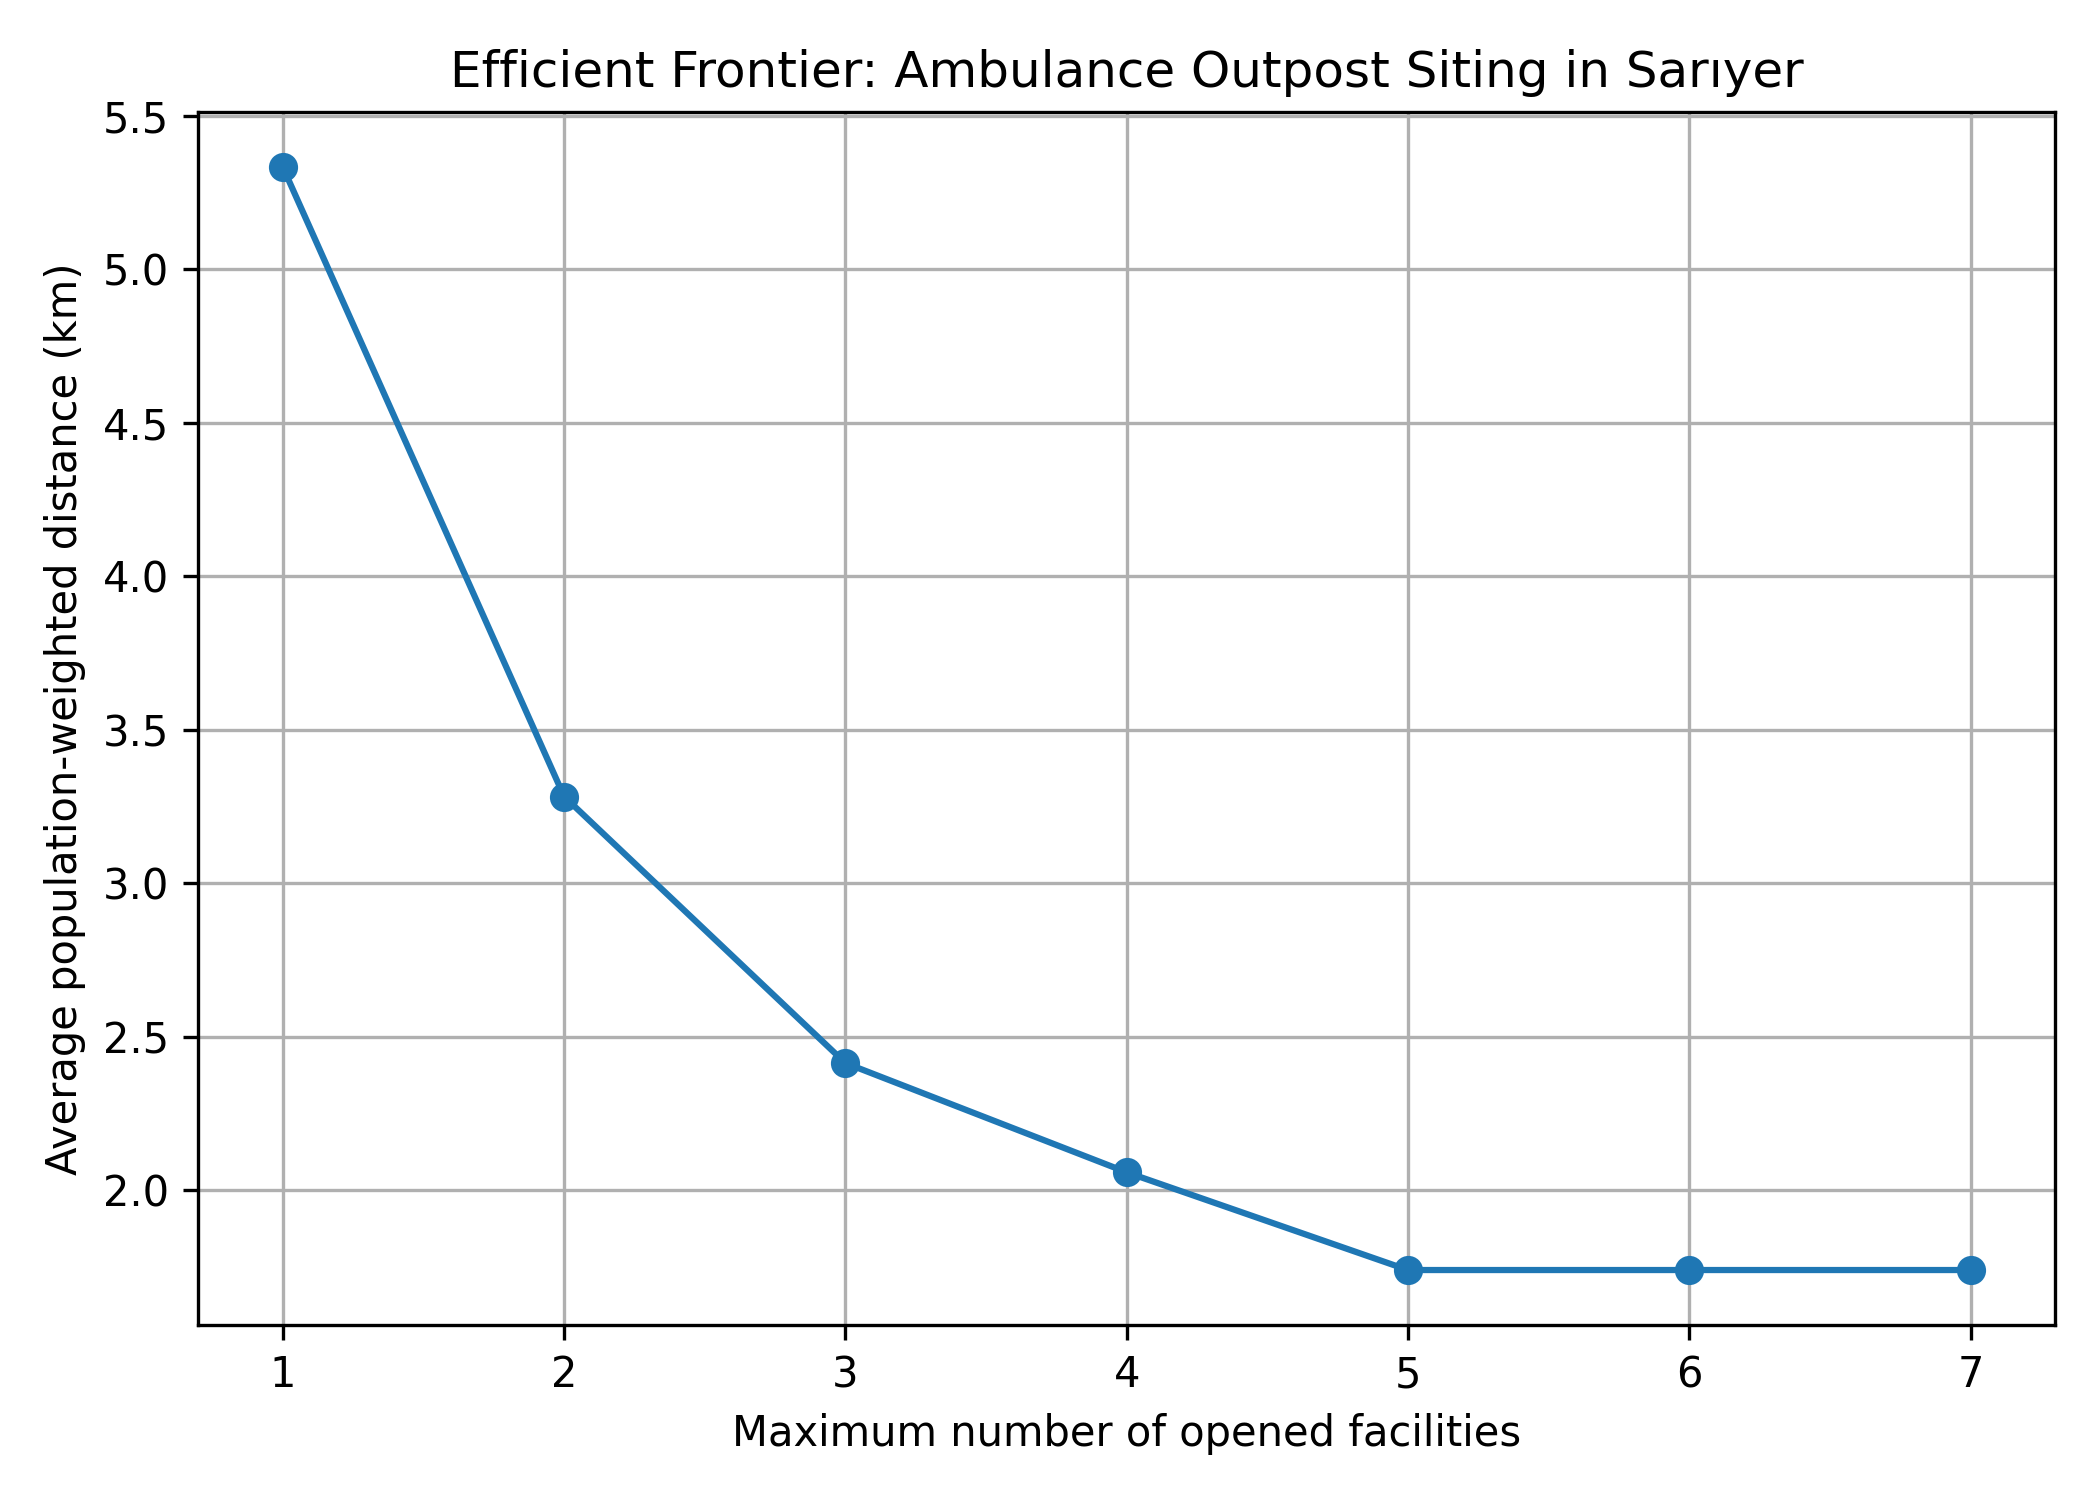
\includegraphics[width=0.75\textwidth]{../outputs/efficient_frontier_seed.png}
\caption{Efficient frontier for ambulance outpost siting in Sar{\i}yer}
\label{fig:frontier}
\end{figure}

\section{Recommended Solution}

The recommended solution is to open four facilities:

\[
\{F2, F3, F6, F7\}
\]

This solution provides a strong practical compromise.
Compared with three facilities, opening the fourth facility reduces the maximum assigned distance from approximately 5.0 km to 3.6 km.
The fifth facility further improves the average distance, but the improvement is smaller relative to the additional infrastructure requirement.

\begin{table}[H]
\centering
\caption{Recommended assignments for MaxFac = 4}
\label{tab:assignments}
\begin{tabularx}{\textwidth}{l l r}
\toprule
Demand Neighborhood & Assigned Facility & Distance (km) \\
\midrule
Ayazaga & F3 & 0.4 \\
Zekeriyakoy & F7 & 1.8 \\
Resitpasa & F3 & 3.4 \\
Tarabya & F2 & 3.4 \\
Fatih Sultan Mehmet & F2 & 3.6 \\
Istinye & F2 & 0.4 \\
Yenikoy & F2 & 2.0 \\
Ferahevler & F2 & 2.8 \\
Maden & F6 & 2.4 \\
Merkez & F6 & 2.3 \\
\bottomrule
\end{tabularx}
\end{table}

\section{Limitations}

This project is a district-scale planning model, not an official EMS deployment plan.
The model uses population as a proxy for EMS demand, whereas real ambulance demand depends on call histories, age distribution, health conditions, time of day, and traffic.
The seed distance matrix should ideally be replaced by live OSRM or openrouteservice driving distances before final submission.

\section{Conclusion}

The analysis shows that an equity-aware ambulance outpost siting model can be implemented for Sar{\i}yer using public data and open-source tools.
The recommended four-facility solution improves both efficiency and equity, while avoiding unnecessary facility expansion.
This makes it a suitable practical recommendation for the course project.

\bibliographystyle{plain}
\bibliography{references}

\end{document}